\section{Реконструкция треков частиц}

Хотя детекторы и аппаратура NA64 технически не ограничивают
регистрацию событий с высокой множественностью треков,
алгоритмическая база представленная одними лишь алгоритмами
подгонки треков недостаточна для надёжной идентификации
и измерения импульса частиц, и применяется для оценки средней
картины. На рисунке~\ref{fig:muon-momenta-test-histogram}
показан спектр мюонов реконструированных при помощи
алгоритма DAF~\cite{daf-track-fitting} при высокой
интенсивности (примерно $10^6$ мюонов в секунду).

Детекторы и система сбора данных NA64 принципиально способны
регистрировать события с высокой множественностью треков
(до нескольких сотен). Однако, без применения алгоритмов
предварительного выбора гипотез, восстановление
трека алгоритмами типа DAF позволяет получить усреднённое представление
о треках частиц, с потерей существенной части физической информации.
На рисунке~\ref{fig:muon-momenta-test-histogram}
приведён спектр мюонов, реконструированных с помощью алгоритма
DAF при высокой интенсивности пучка
(порядка $10^6$ мюонов в секунду).
\begin{figure}[h]
    \centering
    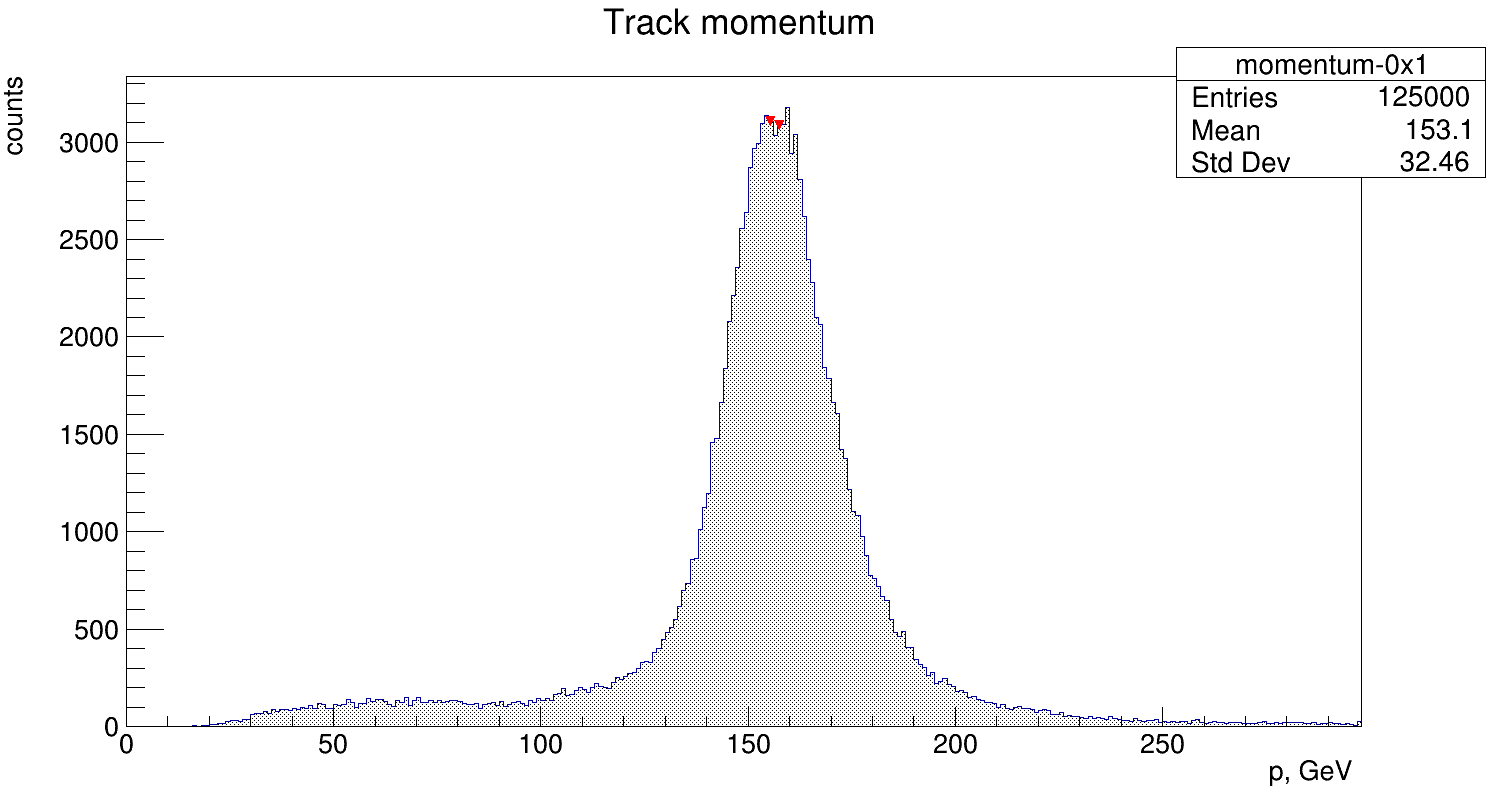
\includegraphics[width=0.65\linewidth]{images//illustrative/momentum-reco-example.png}
    \caption{Спектр мюонов реконструированных алгоритмом DAF без
    предварительного выбора гипотез}
    \label{fig:muon-momenta-test-histogram}
\end{figure}
Пьедестал спектра в основном соответствует случайной сходимости
алгоритма на правдоподобных комбинациях координатных измерений,
без учёта конкурирующих гипотез.

Использование алгоритма CATS для выделения треков частиц
позволяет эффективно исключить некорректные гипотезы, согласно
некоторому геометрическому критерию. При заданной принадлежности
объектов $h_p,h_q,h_r$ идущим по порядку
слоям $h_p\in l_{i-1}, h_i \in l_i, h_p\in l_{i+1}$ критерий $F(h_{p}, h_q, h_{r}) \in [0,1]$ может включать произвольное условие.

\subsection{Результаты CATS(C) на модели данных Belle~II}

В качестве примера, помимо простейшего теста на принадлежность угла
$\angle(h_p,h_q),(h_q,h_r)$ заданному диапазону, можно рассмотреть
постановку задачи в соленаодиальном поле баррельной части коллайдерного
детектора, в рамках которой функция-фильтр $F$ должна проверять
какую-нибудь характеристику спиральной траектории. Например, в цилиндрической системе
координат $(\rho, \phi, z)$, выбирая попарные комбинации из триплета $h_{p}, h_q, h_{r}$,
можно проверять шаг $\lambda_{ij} = \Delta z_{ij}/\Delta \phi_{ij}$
на приблизительное равенство относительно некоторого порога $\epsilon$:
\begin{align}
    F(h_{p}, h_q, h_{r}) = |\lambda_{12} / \lambda_{23} - 1| <\epsilon ~
    \wedge |\lambda_{12} / \lambda_{13} - 1| <\epsilon.
\end{align}

Результаты моделирования в геометрии Belle~II~\cite{belle-ii} изображены на
рисунке~\ref{fig:belle-ii-mc-event}.
\begin{figure}[ht]
    \centering
    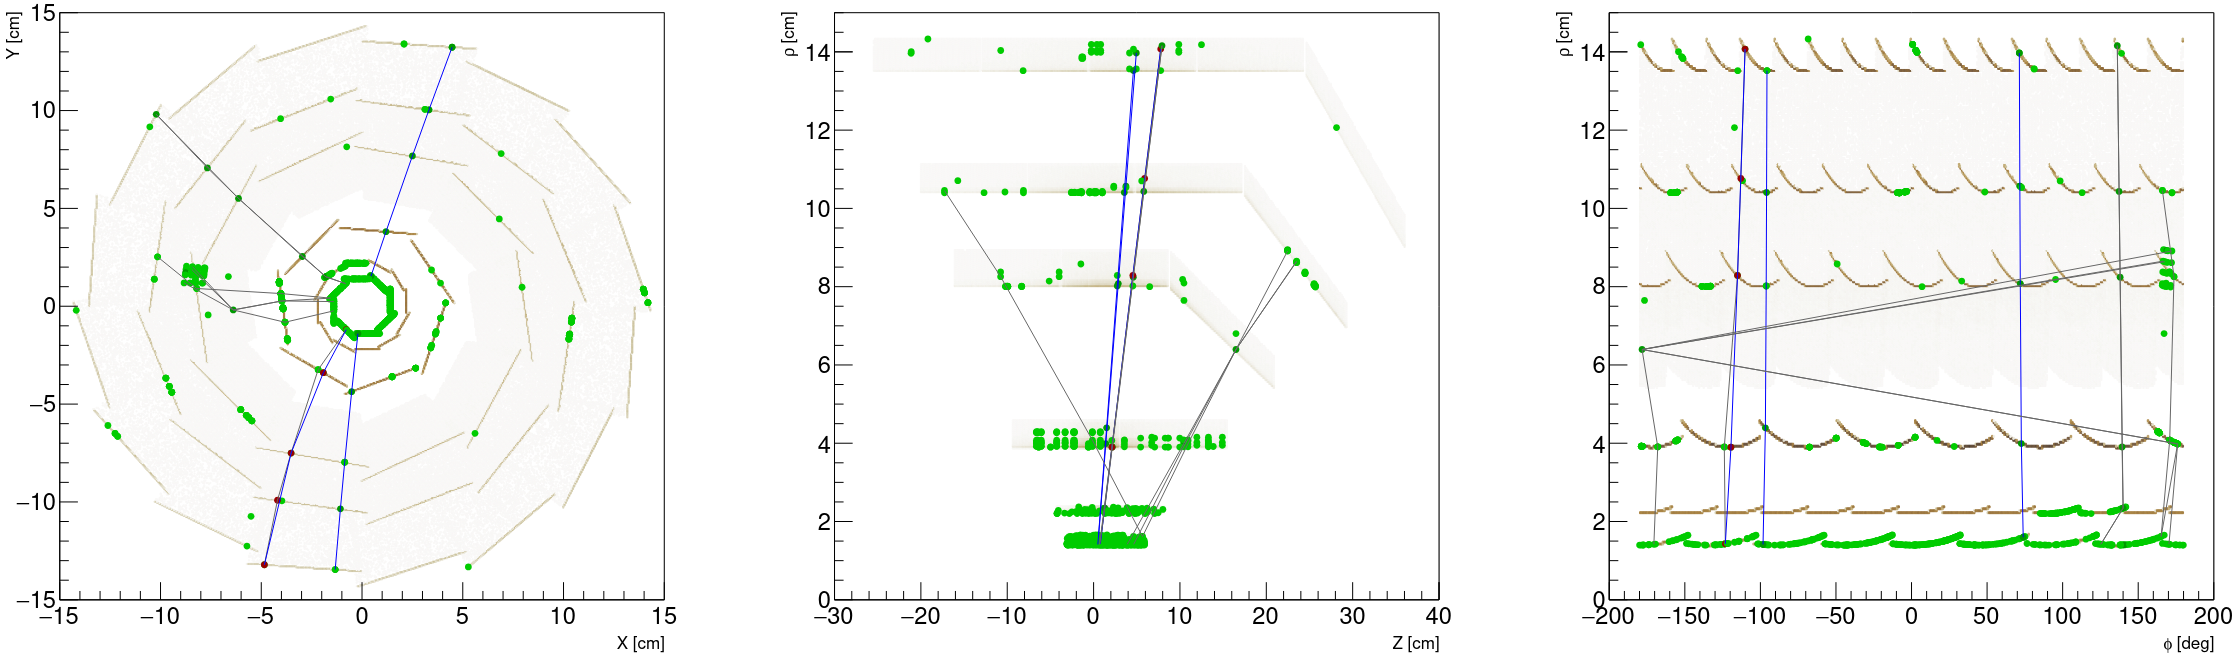
\includegraphics[width=1\linewidth]{images//illustrative/belle-ii-mc-event.png}
    \caption{Результат применения реализации CATS(C) на данных \acrshort{mc}-моделирования
    одного сособытия геометрии детектора Belle II~\cite{belle-ii} 
    (автор -- С.~Герасимов}
    \label{fig:belle-ii-mc-event}
\end{figure}
Поверх схематичного изображения детекторов
внутреннего и внешнего трекера зелёным нанесены точки, соответствующие
измерениям детекторов $h$, синими линиями соединены найденные треки,
соответствующие истинным траекториям, реконструированным алгоритмом;
серым -- комбинации отвечающие ложным гипотезам.

\subsection{Результаты CATS(C) данных NA64mu}

Результаты применения алгоритма для реконструкции треков NA64mu приведены на
рисунке~\ref{fig:cats-impact-na64}.
\begin{figure}[ht]
    \centering
    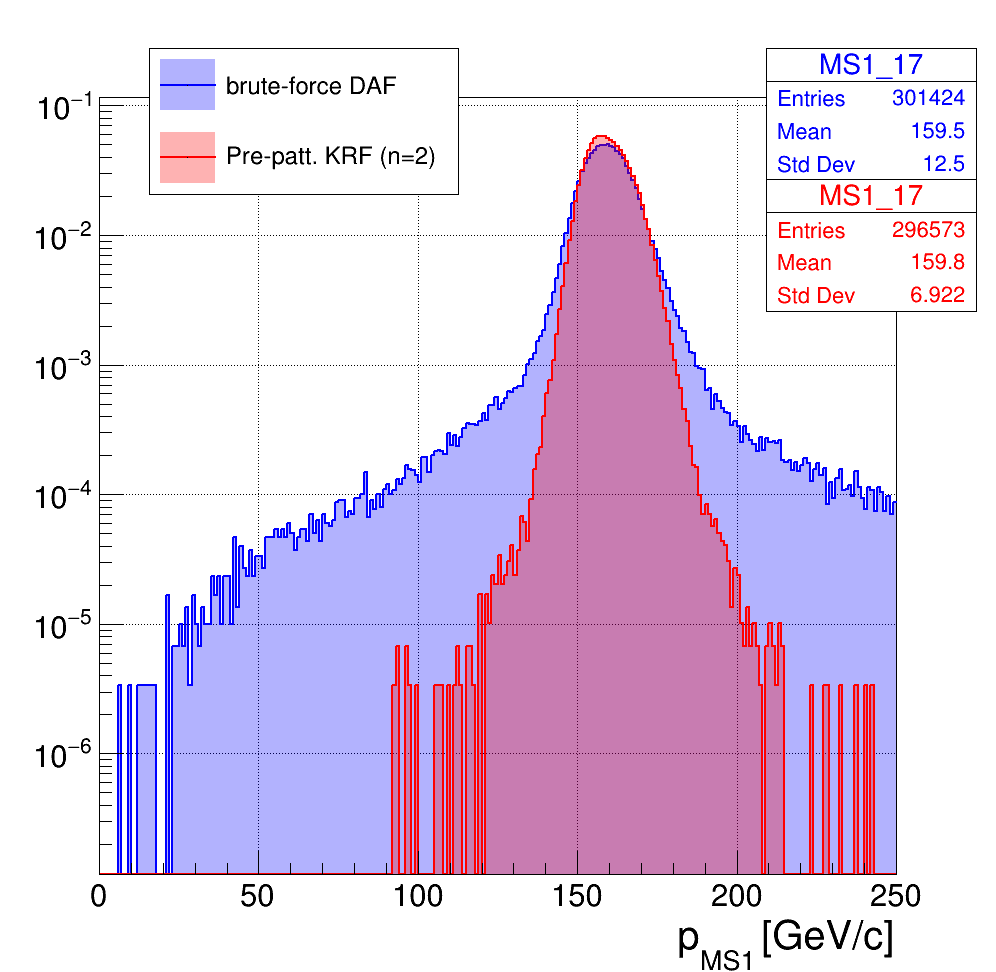
\includegraphics[width=0.49\linewidth]{images//illustrative/catsc-impact.png}
    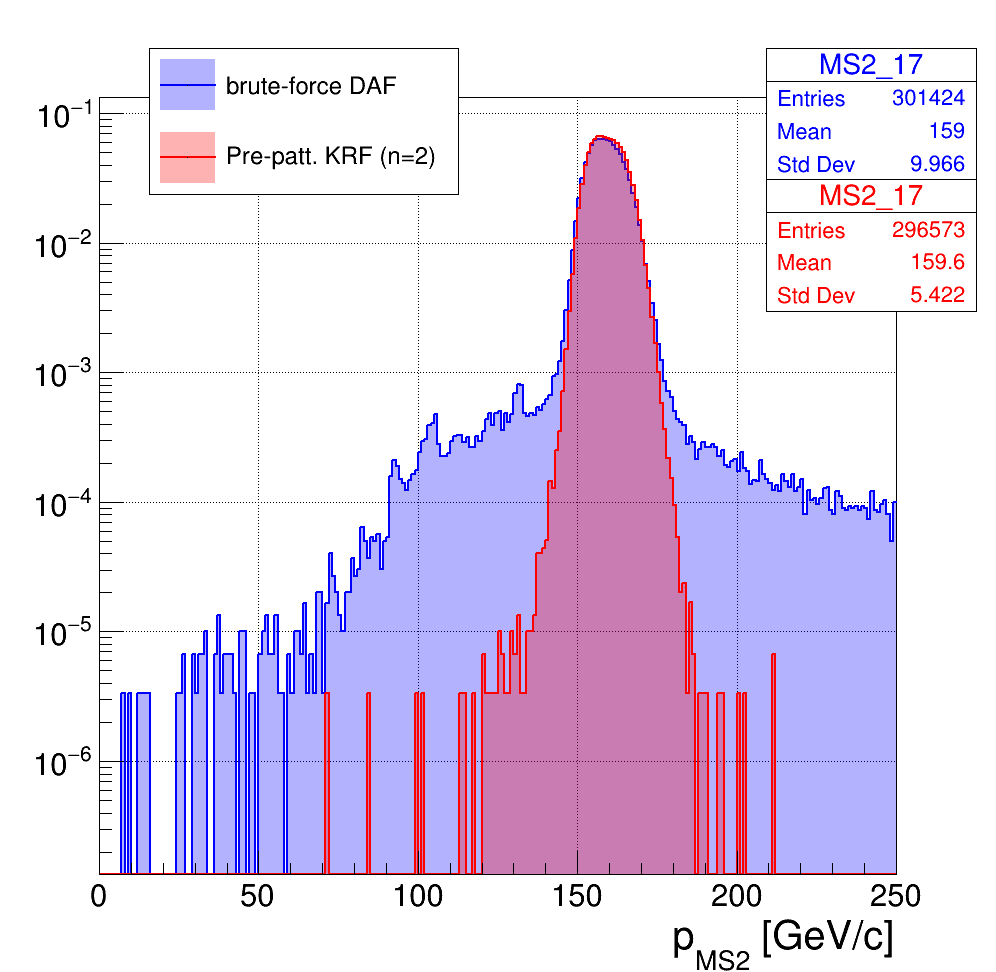
\includegraphics[width=0.49\linewidth]{images//illustrative/catsc-impact-2.png}
    \caption{Распределение импульсов частиц NA64mu реконструированных при
    помощи DAF без применения CATS(C) и при помощи KRF после CATS(C)
    до (MS1) и после (MS2) основного магнита спектрометра NA64mu~(автор -- M.~Tuzi)}
    \label{fig:cats-impact-na64}
\end{figure}
В постановке NA64mu применение алгоритма для предварительного отбора гипотез треков
особенно важно, поскольку участок установки MS2 находится после электромагнитного
калориметра, и трекер должен разрешать траектории при повышенной
загрузке (в среднем $\simeq 10$ треков на событие против $\simeq 1.4$ в MS1)
от вторичных частиц после ECAL.

При консервативной оценке пороги для углов или спирального шага
регулируют в основном количество избыточных гипотез найденных алгоритмом, которые
затем отсеивают при подгонке треков и проверки более строгих гипотез. Избыточные
гипотезы можно ограничить на основе оценок порогов полученных с
применением \acrshort{mc}-моделирования, или при помощи консервативных
геометрических оценок.

В частности, на рисунке \ref{fig:belle-ii-catsc} приведены результаты моделирования
для Belle~II, откуда для заданного уровня статистической значимости можно получить
ограничения на значения различных порогов функции-фильтра. На рисунке зелёным цветом
выделены значения, соответствующие истинным трекам (которые размываются благодаря
рассеянию в детекторах), комбинаторный фон обозначен жёлтым.

\begin{figure}
    \centering
    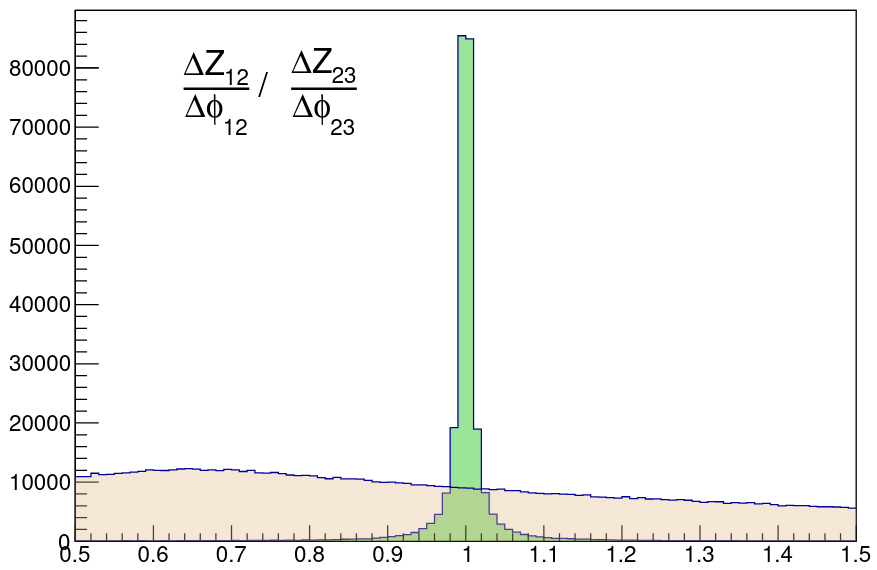
\includegraphics[width=0.32\linewidth]{images//illustrative/pitch-ratios.png}
    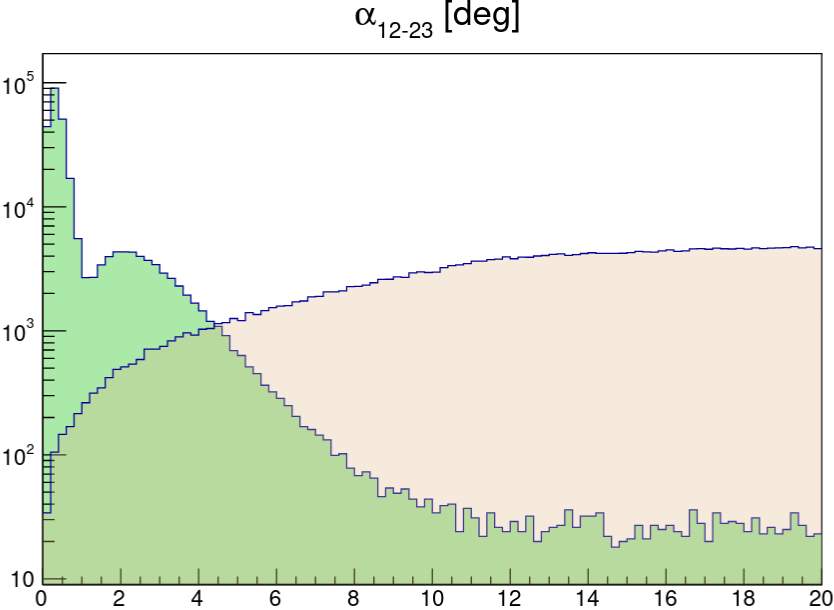
\includegraphics[width=0.32\linewidth]{images//illustrative/belle-ii-catsc-opening-angle.png}
    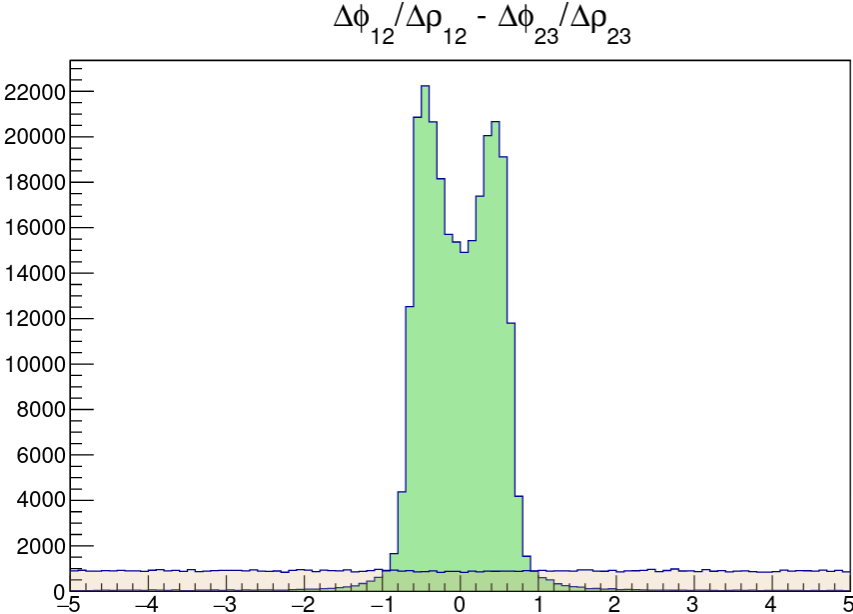
\includegraphics[width=0.32\linewidth]{images//illustrative/belle-ii-catsc-pitch-delta.png}
    \caption{Распределения отношения спирального шага $\lambda_{12}/\lambda_{23}$,
    продольного угла в триплете $\alpha_{12-23}$ и разницы спиральных шагов
    $\lambda_{12} - \lambda_{23}$ по результатам \acrshort{mc}-моделирования
    Belle~II для оценки мощности критерия~(С.~Герасимов)}
    \label{fig:belle-ii-catsc}
\end{figure}

В некоторых случая можно прибегнуть к упрощённому рассмотрению.
Рисунок~\ref{fig:na64-cutoff-angle} иллюстрирует распределение углов
для допустимых триплетов $h$ в пределах $3\sigma$, где $\sigma$ -- пространственное
разрешение одной станции. Видна существенная (вплоть до кратности $\times5$) разница
углового порога.
\begin{figure}[ht]
    \centering
    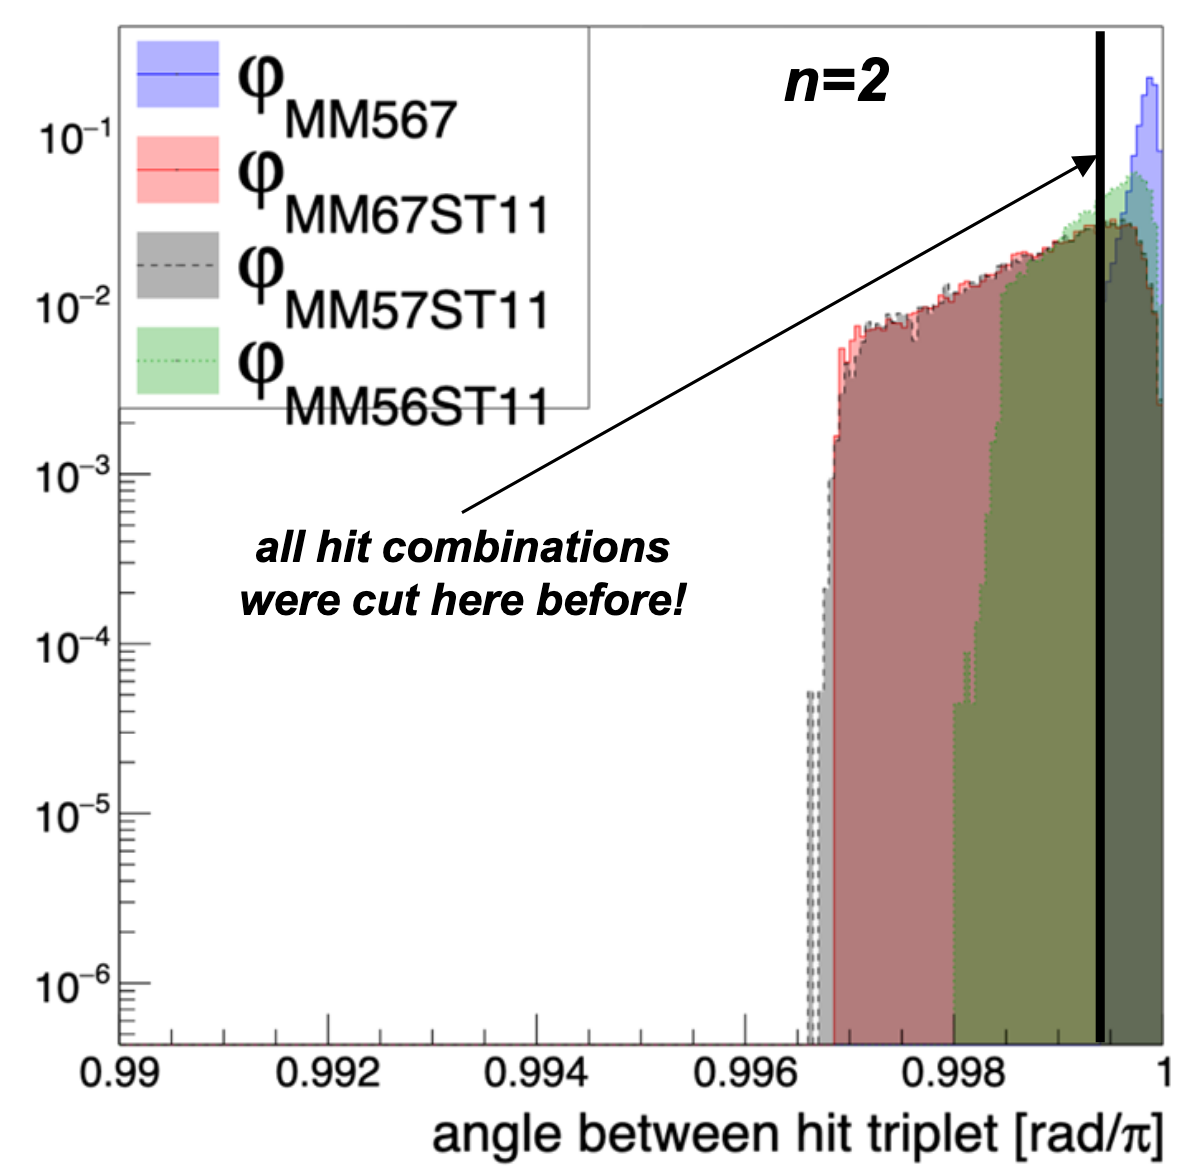
\includegraphics[width=0.5\linewidth]{images//illustrative/na64-cutoff-effic.png}
    \caption{Распределение углов для всех возможных комбинаций при учёте разрешения
    отдельных станций трекера MS2 NA64mu~(M.Tuzi)}
    \label{fig:na64-cutoff-angle}
\end{figure}

\subsection{Количественные оценки качества восстановления треков}

Задача восстановления треков частиц по данным зачастую формулируется
как минимизация функционала, в котором в качестве метрического значения
выбирается величина, пропорциональная отклонению ожидаемых значений
от фактически измеренных. Для многих детекторов статистика таких
отклонений (ошибок), отнесённых к абсолютному разрешению детектора,
подчиняется распределению~$\chi^2$.

На рисунке~\ref{fig:na64-muon-p-value-distribution} показаны распределения $p$-значений
(интегральных вероятностей $\chi^2$) в плече MS1. Вид этого распределения
используется для косвенной оценки качества работы трекера. В случае полного
соответствия фактических разрешений детекторов установки номинальным
распределение должно быть плоским. Увеличение популяции справа
($p_{\chi^2} \rightarrow 1{,}0$) означает, что разрешение одной или нескольких
станций оценивается пессимистически (фактическое меньше ожидаемого).
\begin{figure}[ht]
    \centering
    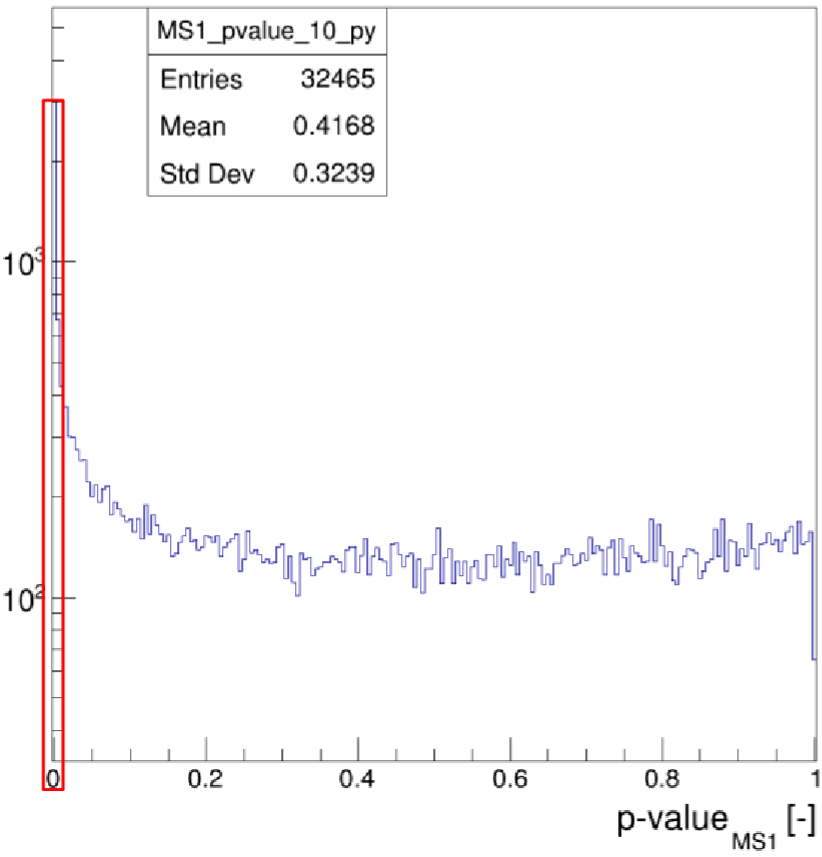
\includegraphics[width=0.5\linewidth]{images/na64-ms1-p-value-before.png}
%    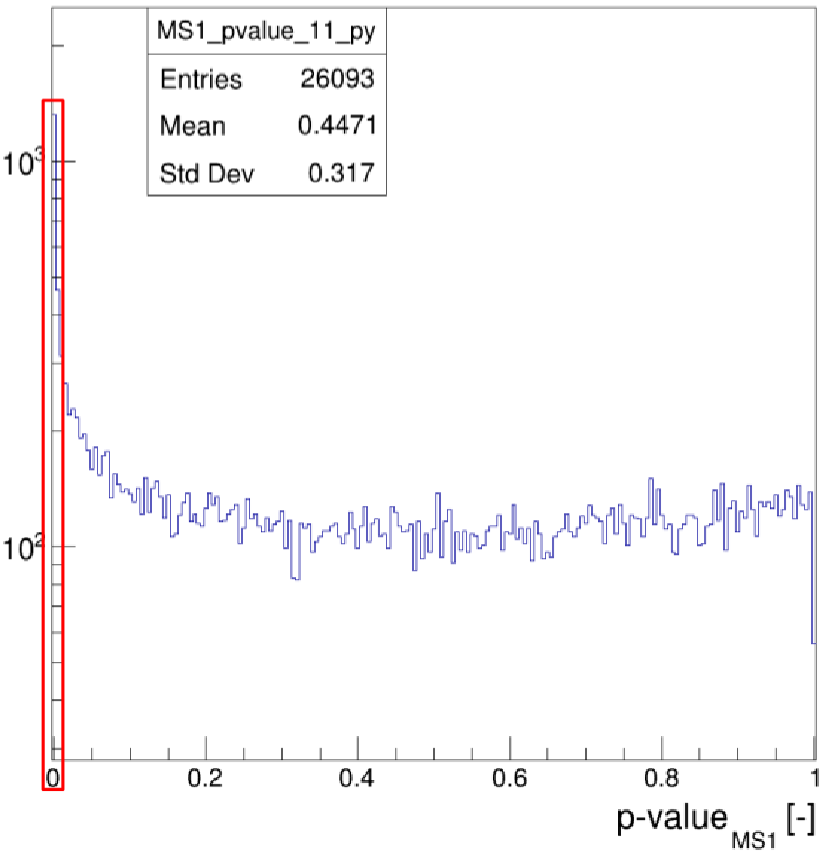
\includegraphics[width=0.5\linewidth]{na64-muon-p-value-ms1-dist-after.png}
    \caption{Распределение $p_{\chi^2}$ реконструированных треков в плече MS1 мюонного спектрометра NA64 после выравнивания~(M.Tuzi)}
    \label{fig:na64-muon-p-value-distribution}
\end{figure}

Наблюдаемое на рисунке увеличение популяции слева свидетельствует о наличии факторов,
неучтённых моделью трека: неудовлетворительного геометрического выравнивания, снижения
эффективности за счёт дефектов детектора, большего вклада множественного рассеяния и т.~д.
На приведённой гистограмме около 7\% треков отклоняются как не соответствующие уровню
значимости $\alpha = 0{,}01$.

%\begin{figure}[ht]
%    \centering
%    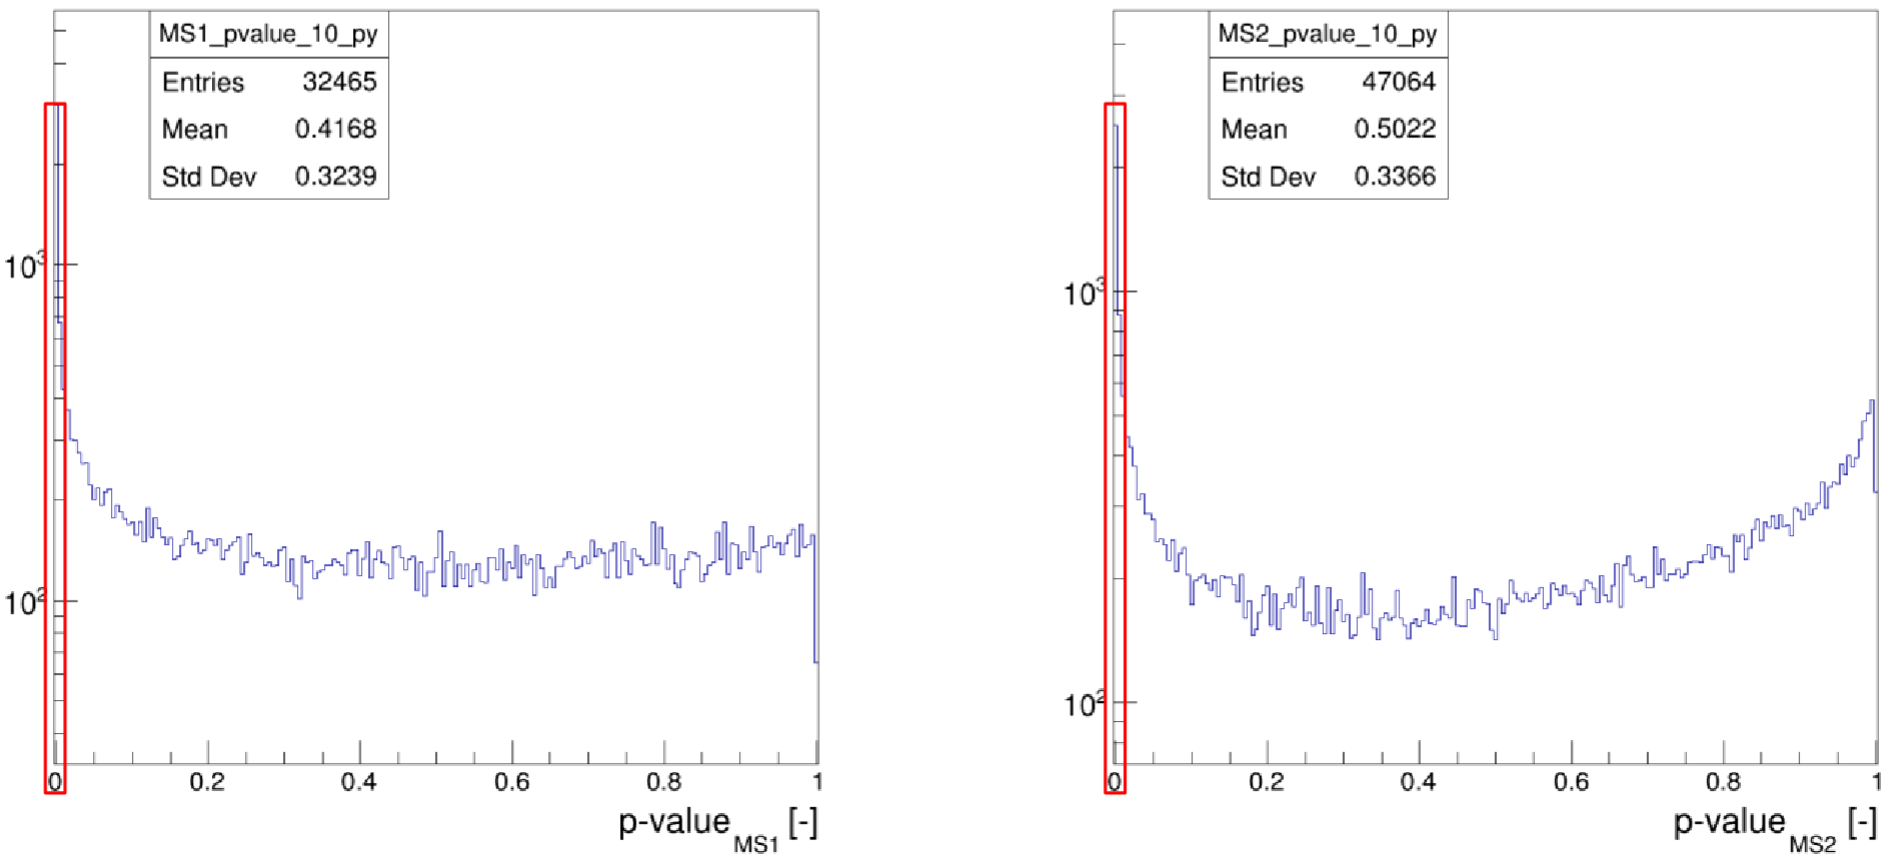
\includegraphics[width=1\linewidth]{images//illustrative/na64-p-value-before-truly.png}
%    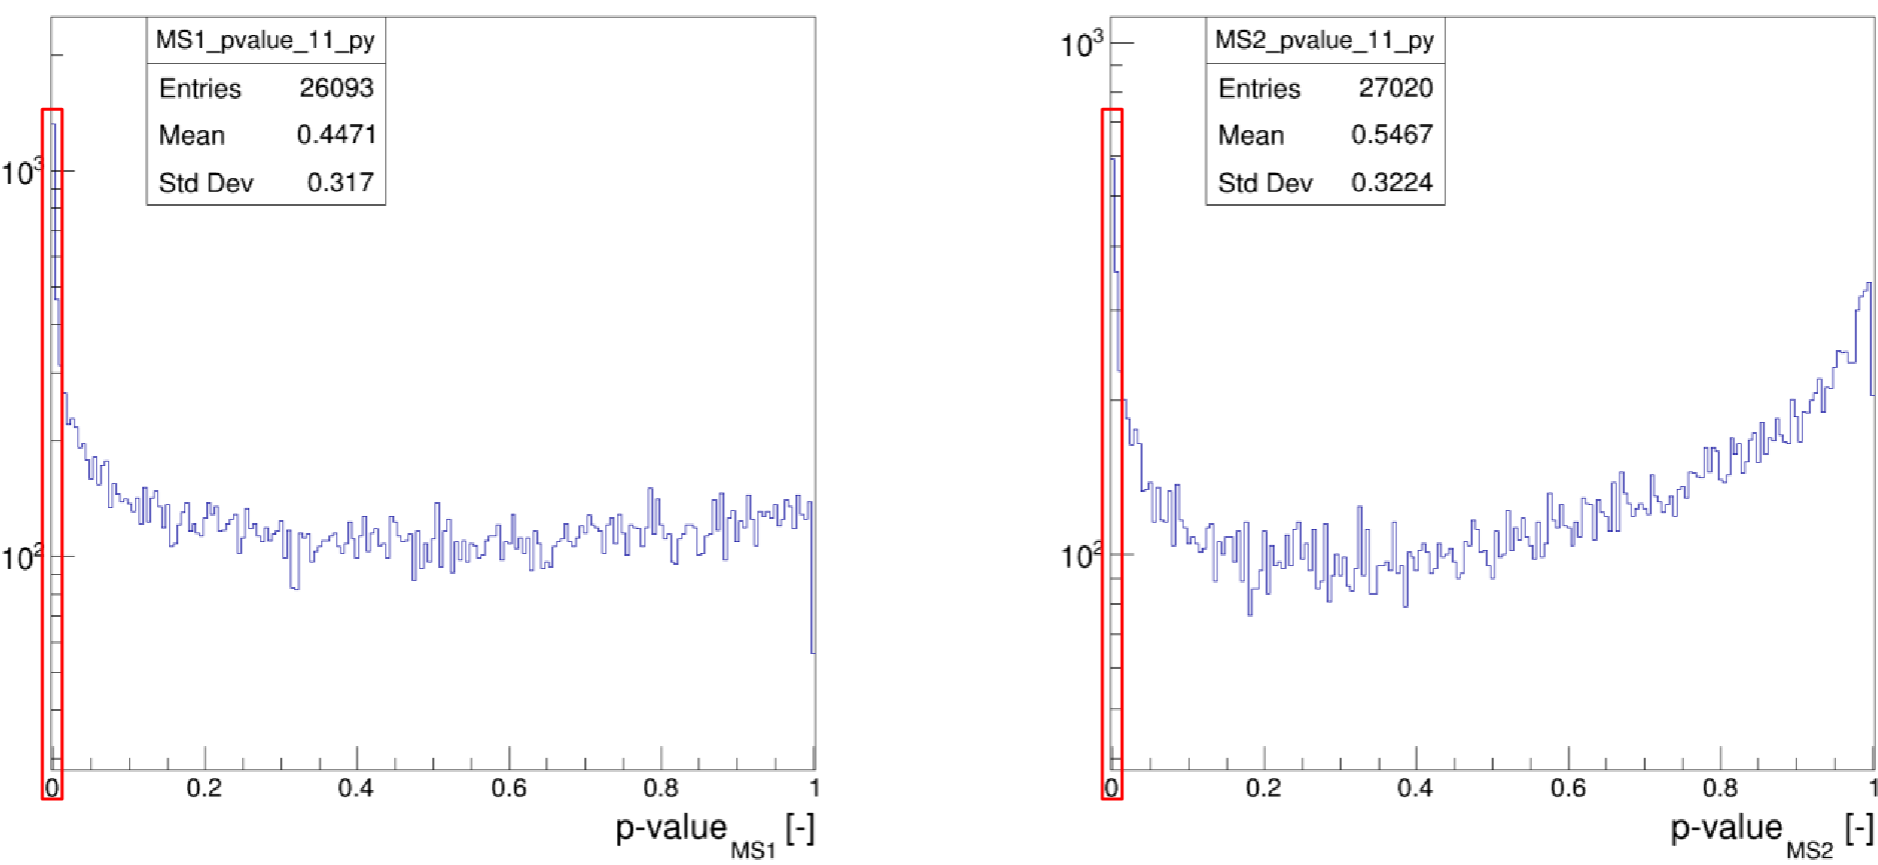
\includegraphics[width=1\linewidth]{images//illustrative/na64-pvalue-before.png}
%    \caption{Распределение $p_{\chi^2}$ реконструированных треков для плечей мюонного спектрометра NA64 до и после учёта wire layout~(M.Tuzi)}
%    \label{fig:na64-muon-p-value-distribution}
%\end{figure}

Важным фактором, влияющим на качество восстановления треков, является
соответствие предполагаемых положений детекторов фактическим. Для
оценки этого соответствия в случае индивидуальных детекторов строят
распределения координатных невязок (англ. \emph{residuals}) в
системе локальных координат, связанной с детектором.
Для стриповых детекторов (измеряющих координату в одном направлении)
используют одно направление ($u$), выбираемое соответствующим измеряемой
координате, второе обычно перпендикулярно ему.

При ориентации плоскости перпендикулярно пучку распределение невязок
характеризует ошибку в определении позиции центра
координатной плоскости детектора в поперечных координатах (вдоль $u$).
Для получения более детализированной картины строят
распределение $\delta u/dv$, естественно характеризующее ошибку в определении
угла поворота, перпендикулярного направлению пучка. Распределение
$\delta u/du$ характеризует ошибку в определении продольной координаты.

На рисунке~\ref{fig:residuals-example} показан пример комплексного
графика, характеризующего распределение невязок $\delta u$ против $v$.
\begin{figure}[ht]
    \centering
    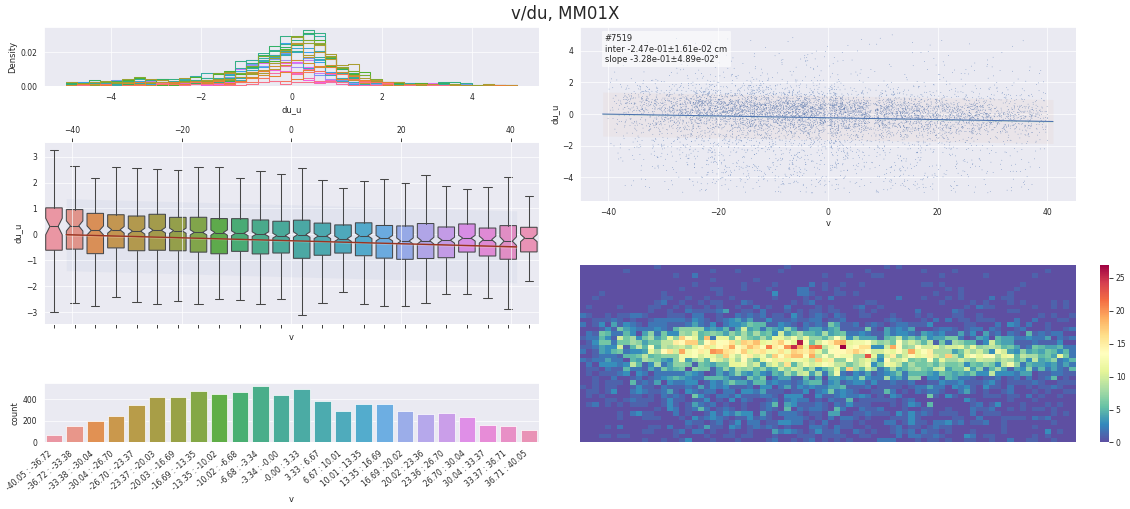
\includegraphics[width=0.95\linewidth]{images/illustrative/alignment-example.png}
    \caption{Комплексный график иллюстрирующий распределение координатных
    невязок $\delta u /v$ для плоскости X первой станци MicroMega}
    \label{fig:residuals-example}
\end{figure}

Такое изображение координатных невязок можно использовать, в частности,
в процедуре выравнивания детекторов по \emph{несмещённым} невязкам, когда
среди всего набора выбирается пара опорных детекторов $P_1,~P_2$, по отношению
к которым производят итеративное выравнивание. Включая в процедуру
реконструкции по одному детектору последовательно, для каждого уточняют
значения позиций и углов на основе распределений подобных изображённым
на рисунке~\ref{fig:residuals-example} при условии что рассматриваемый
в данный момент детектор не используется для реконструкции треков (однако,
программный комплекс расчитывает для него координатные невязки).

Подобные изображения координатных невязок используются, в частности,
в процедуре выравнивания детекторов по \emph{несмещённым} невязкам.
В такой процедуре из всего набора выбирается пара опорных детекторов,
относительно которых проводится итеративное выравнивание.
Для каждого отдельного детектора уточняют положения и углы на основе распределений,
подобных показанным на рисунке~\ref{fig:residuals-example}, при условии,
что данный детектор не используется для реконструкции треков (однако
программный комплекс вычисляет для него координатные невязки). После
выравнивания очередного детектора, он добавляется к опорным, и переходят
к следующему.

Процедура выравнивания по \emph{смещённым} невязкам, напротив,
предполагает включение всех корректируемых детекторов в реконструкцию трека.
В этом случае линеаризованные невязки образуют блочную матрицу,
которую можно использовать для решения СЛАУ.

В рассматриваемом программном окружении реализованы инструменты
для обеих процедур физического выравнивания и оценивания качества
реконструкции треков частиц. Инструменты для выравнивания по
несмещённым невязкам (графики и регрессионные модели) реализованы
в парадигме отдельных обработчиков ковейерного паттерна, выравнивание
по смещённым невязкам реализовано в виде специализированных
обработчиков и специализированной утилиты для помещения их вывода
на вход процедуры обращения блочных матрицы
Millipede~II~\cite{millipede-blobel2009}.
